\chapter{Results}
\label{chap:results_method_development}

\section{Haemocyte medium}
The following section presents results from two experiments that were conducted to explore the suitability of three haemocyte media for applications in flow cytometric assays. They are compared with regard to their ability to inhibit haemocyte aggregation, without affecting the viability of haemocytes.

\subsection{Inhibition of haemocyte aggregation}
The proportions of aggregated haemocytes in \acrshort{mpss}, \acrshort{acb} and \acrshort{mas} are plotted against time post-withdrawal in Figure \ref{fig:aggregation}, together with their predicted mean proportions, or more accurately: the predicted proportion of aggregated haemocytes in mussels with random effects $\gamma_{0i}$ and $\gamma_{1i}$ = 0. Predictions were made from the estimated fixed effects in order to address the marginal effect of "Buffer" on the population-averaged proportions. The estimated regression coefficients of the generalized linear mixed effect model is presented in Table \ref{tb:regression_table}, while the fixed effect sub-models are shown in (\ref{eq:mixed_submodels}).

\begin{equation}
    \label{eq:mixed_submodels}
    y_{ij} = \begin{cases}
        \dfrac{1}{1 + e^{-(-1.7192 + 0.5516 \times log(t_{ij}))}},  & i \: \text{in MPSS group}, \\
        \dfrac{1}{1 + e^{-(-6.9842 + 1.8400 \times log(t_{ij}))}},  & i \: \text{in ACB group}, \\
        \dfrac{1}{1 + e^{-(-7.7198 + 2.0138 \times log(t_{ij}))}},  & i \: \text{in MAS group} \\
    \end{cases}
\end{equation}

Figure \ref{fig:aggregation}D unambiguously demonstrates that both \acrshort{acb} and \acrshort{mas} exerted an immediate decelerating effect on the rate of haemocyte aggregation. This inhibitory effect is evident from the estimated differences in slopes and intercepts from the MPSS sub-model, which were significantly different from zero (see Table \ref{tb:regression_table}). Since the effect sizes are a bit challenging to interpret from the isolated coefficients, the linear predictors of the three sub-models are evaluated on link scale in Figure \ref{fig:LogOdds}, i.e. as predictors for the log odds of the proportion of aggregated haemocytes ($log P(y_{ij} = 1) / P(y_{ij} = 0)$).

\begin{figure}[!ht]
    \centering
    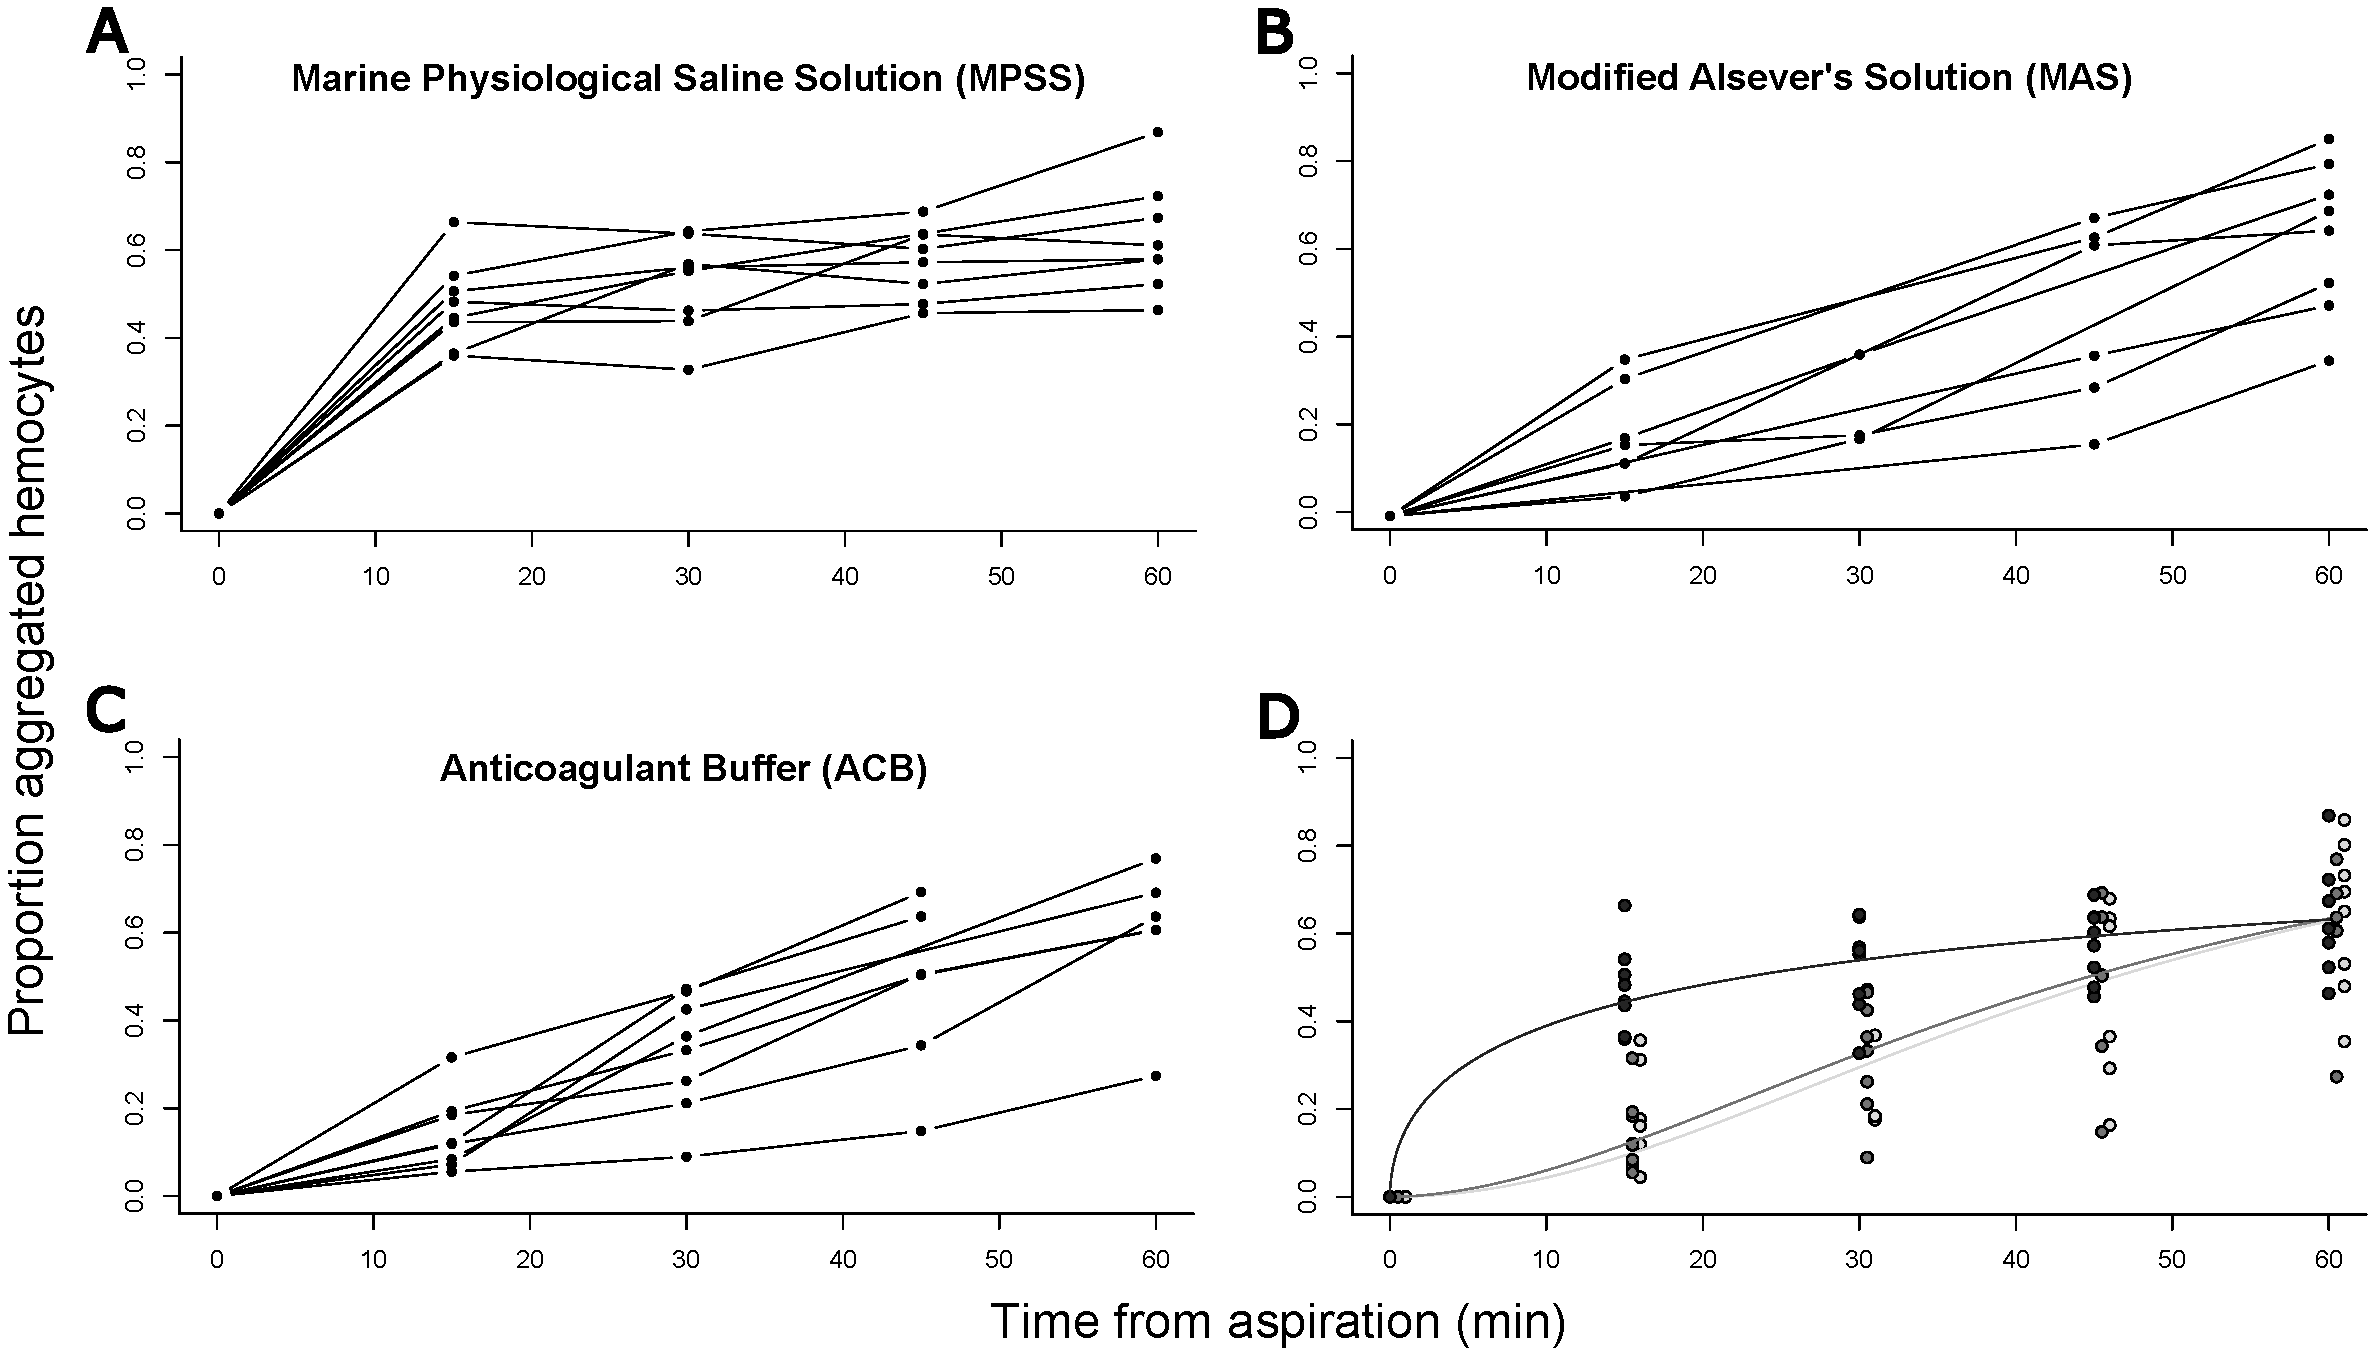
\includegraphics[width=1.0\textwidth]{figures/Method development/Propagg x4 plot.pdf}
    \caption{\textbf{Inhibition of hemocyte aggregation from withdrawing samples into three different anticoagulant buffers.} The proportion of aggregated hemocytes is plotted against time from haemolymph withdrawal after diluting samples in an equal volume of \textbf{A)} Marine Physiological Saline Solution (\acrshort{mpss}, n=8), \textbf{B)} Modified Alsever's Solution (\acrshort{mas}, n=8) or \textbf{C)} Anticoagulant Buffer (\acrshort{acb}, n=8).  \textbf{D)} The same data is combined into one scatter-plot with regression curves representing the mean proportions of aggregated haemocytes in \acrshort{mpss} (\protect\darkgraycircle), \acrshort{mas} (\protect\lysegraacircle) and \acrshort{acb} (\protect\graycircle), as predicted from the fitted mixed logistic regression model. Note that data-points have been jittered on the x-axis to prevent overlap.}
    \label{fig:aggregation}
\end{figure}

\begin{table}[H]
	\centering
	\caption{Parameter estimates of the fitted mixed logistic regression model and their 95\% confidence intervals. Marginal and conditional R$^{2}$-values are presented as parameters of model fit, together with the model's residual deviance.}
	\label{tb:regression_table}
	\begin{tabular}{llllc}
        \toprule
	\textbf{Covariate} & \textbf{Symbol} & \textbf{Estimate$^{b}$} & \textbf{95\% CI$^{a}$} & \textbf{S.E.}\\
		\midrule
  \emph{Intercept}                          & $\alpha_1$ & -1.72*     & [-3.24, -0.202] & 0.740 \\
  \emph{log(t)}                             & $\beta_1$  & 0.552**    & [0.189, 0.915]  & 0.177 \\
  \emph{Buffer$_{ACB}$}                     & $\alpha_2$ & -5.27***   & [-7.41, -3.11]  & 1.05  \\
  \emph{Buffer$_{MAS}$}                     & $\alpha_3$ & -6.00***   & [-8.18, -3.86]  & 1.06  \\
  \emph{log(t)} $\cdot$ \emph{Buffer$_{ACB}$} & $\beta_2$& 1.29***    & [0.775, 1.80]   & 0.251 \\
  \emph{log(t)} $\cdot$ \emph{Buffer$_{MAS}$} & $\beta_3$& 1.46***    & [0.950, 1.98]   & 0.253 \\
  \emph{SD}$(\gamma_{0i})$                  & $\tau_0^2$ & 2.09       & [1.57, 2.91]    & -     \\
  \emph{SD}$(\gamma_{1i})$                  & $\tau_1^2$ & 0.500      & [0.379, 0.694]  & -     \\
  &&& \\
  \multicolumn{5}{l}{Marginal R$^{2}$ = 0.87$^{c}$} \\
  \multicolumn{5}{l}{Conditional R$^{2}$ = 0.98$^{c}$} \\
  \multicolumn{5}{l}{Residual deviance: 13498 on 98 degrees of freedom} \\
		\bottomrule
  \multicolumn{5}{l}{\footnotesize $^{a}$Computed 95\% confidence intervals based on Likelihood Ratio Test of the profile likelihood.} \\
  \multicolumn{5}{l}{\footnotesize $^{b}$ *, **, *** indicates statistical significance on 95\%, 99\% and 99.9\% confidence levels, respectively.} \\
  \multicolumn{5}{l}{\footnotesize Confidence levels were obtained from z-statistics of the asymptotic Wald test.} \\
    \multicolumn{5}{l}{\footnotesize $^{c}$Calculated according to the method proposed by Nakagawa and Schielzeth (2013).} \\
	\end{tabular}
\end{table}

\begin{figure}[!ht]
    \centering
    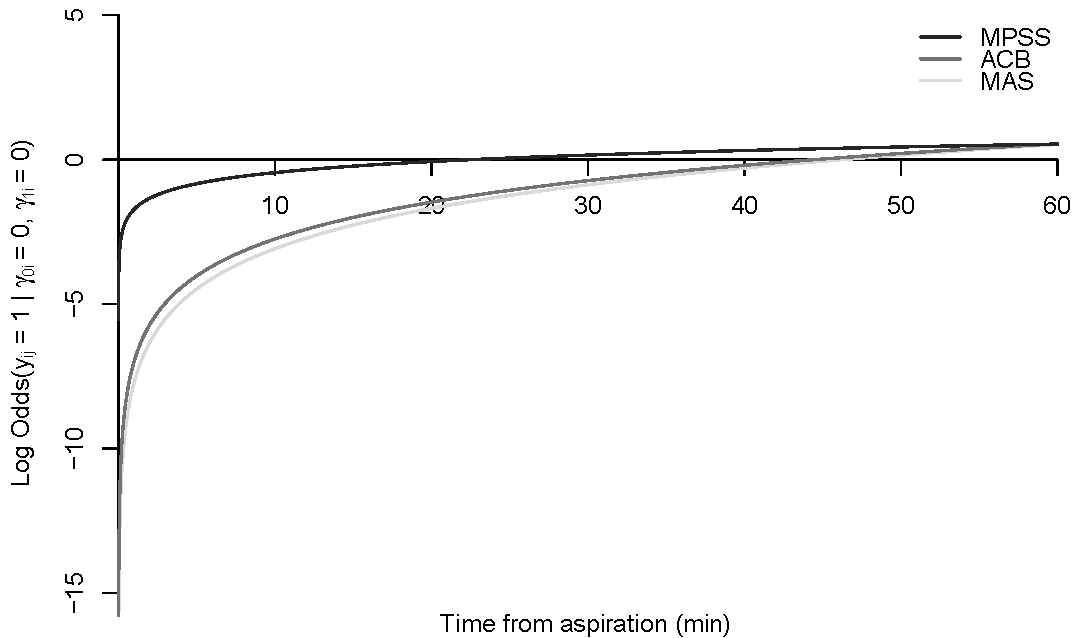
\includegraphics[width=1.0\textwidth]{figures/Method development/Log Odds plot.pdf}
    \caption{The log odds of the proportion of aggregated haemocytes plotted against time (min) after haemolymph withdrawal, when haemolymph samples were withdrawn into Marine Physiological Saline Solution (MPSS), Anticoagulant Buffer (ACB) or Modified Alsever's Solution (MAS). The three curves illustrates the logit-scale predictors of the fitted mixed logistic regression model for the three buffers.}
    \label{fig:LogOdds}
\end{figure}

Given the that the predicted proportion of aggregated haemocytes is 0.50 when the log odds is equal to zero, Figure \ref{fig:LogOdds} shows that 1/2 of the haemocytes withdrawn into \acrshort{mpss} had aggregated within 23 minutes post-withdrawal. This interpretation is valid for mussels where the random effects of time; $\gamma_{0i}$ and $\gamma_{1i}$ = 0. For samples withdrawn into \acrshort{acb} or \acrshort{mas} on the other hand, the cells did not achieve this degree of aggregation until 45 and 46 minutes post-withdrawal, respectively. The three log odds curves depicted in Figure \ref{fig:LogOdds} shows that the inhibitory effects of \acrshort{acb} and \acrshort{mas} were modelled through their significantly lower y-intercepts compared to the \acrshort{mpss} sub-model (Table \ref{tb:regression_table}). Since these estimates were significant after accounting for within-mussel correlations (<.001), we can conclude that \acrshort{edta} is an effective haemocyte anticoagulant on the short term.

The effect was largest during the initial 15-20 minutes, before the degree of aggregation slowly approached that of \acrshort{mpss} around 60 minutes post-withdrawal. In haemolymph samples withdrawn into \acrshort{acb} or \acrshort{mas}, the mean proportions of aggregated haemocytes after 15 minutes were 0.14 95\% CI [0.07, 0.22] and  0.20 95\% CI [0.07, 0.32], respectively. There were no significant differences between the buffers with \acrshort{edta}, but both \acrshort{acb} and \acrshort{mas} had significantly lower proportions at this timepoint compared to samples withdrawn into cold \acrshort{mpss} (0.48 95\% CI [0.39, 0.56]).

\subsection{EDTA cytotoxicity}
 The mean percentages of necrotic hemocytes in \acrshort{mpss}, \acrshort{acb} and \acrshort{mas} after 15 minutes, 2 hours and 20 hours incubation are presented in Figure \ref{fig:BufferViability}, with error bars representing 95\% confidence intervals around group means. Within group differences in means at the three incubation periods are presented Table \ref{tb:Paired_ttests}.

\begin{figure}[H]
    \centering
    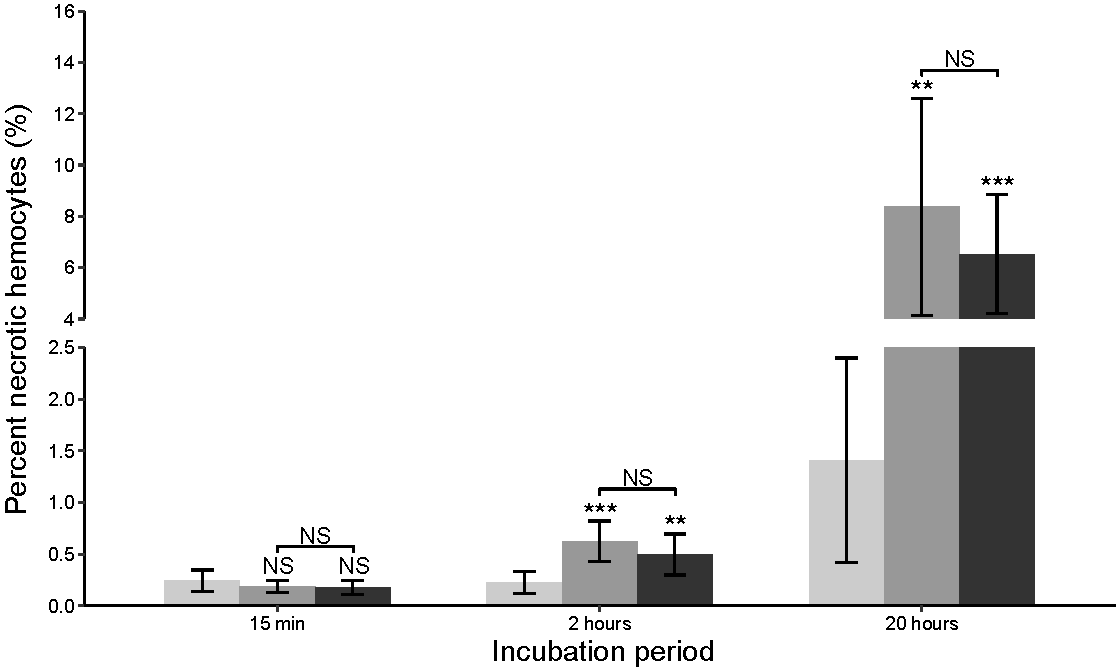
\includegraphics[width=0.75\textwidth]{figures/Method development/EDTA cytotoxicity.pdf}
    \caption{The mean percentages of TO-PRO$^{TM}$-3 Iodide positive hemocytes after 15 minute, 2 hours and 20 hours incubation in Marine Physiological Saline Solution (\, \protect\lysegraabox, \ n=8), Anticoagulant Buffer (\, \protect\customgraybox, \ n=8) and Modified Alsever's Solution (\, \protect\darkgraybox, \ n=8). Error bars represent 95\% confidence intervals around group means, *, **, *** above error bars denotes confidence level of one-tailed two sample t-test comparisons with the \acrshort{mpss} control group, while asterisks above horizontal lines represent \acrshort{acb} vs. \acrshort{mas} comparisons. NS: Not Significant.}
    \label{fig:BufferViability}
\end{figure}

The difference between the negative control group (\acrshort{mpss}) and the two \acrshort{edta}-containing buffers were not significantly different from zero after 15 minute incubation. But as the incubation period was increased to 2 and 20 hours, the percentages of necrotic haemocytes in \acrshort{acb} and \acrshort{mas} increased relative to the negative control group. After 2 hours incubation, there were 0.40\% and 0.27\% more necrotic haemocytes in \acrshort{acb} (t(14) = 4.29, p<.001) and \acrshort{mas} (t(14) = 2.86, p=.006) compared to cold \acrshort{mpss}, respectively. After 20 hours incubation, these differences had increased to 6.96\% (t(14) = 3.78, p=.003) and 5.12\% (t(14) = 4.82, p<.001).

The mean percentage of necrotic haemocytes increased significantly with the incubation period in both MAS and ACB (Table \ref{tb:Paired_ttests}). Since the concentration of EDTA was constant across all timepoints, this increase was dose-dependent as the exposure duration was the only variable factor. There were no significant increase in the percentage of necrotic haemocytes in MPSS from 15 minutes to 2 hours incubation, but a significant increase of 1.184\% was observed after 20 hours (p<.026).

\begin{table}[h!]
\centering
	\caption{Paired two-tailed t-tests were used to assess wether the percentages of necrotic haemocytes increased with incubation time within each group. The difference between means at t = 15 min, 2 hours and 20 hours are presented with 95\% confidence intervals and the belonging p-value.}
	\label{tb:Paired_ttests}
        \resizebox{\linewidth}{!}{
	\begin{tabular}{c|ccccc}
		\toprule
		\multirow{2}{*}{Buffer} & \multicolumn{2}{c}{\textbf{Paired t-test comparison}} & \multirow{2}{*}{Difference (\%)} & \multirow{2}{*}{95\% CI} & \multirow{2}{*}{Pr(T > $\mid$ t $\mid)$} \\
		& Incubation \emph{t} & Incubation \emph{t - 1} & & & \\
		\midrule
     \multirow{2}{*}{MPSS} &  2 hours  &  15 min  & -0.018 & [-0.023, -0.015] & .78 \\
     &  20 hours &  2 hours & 1.184  & [1.157, 1.211]   & .026 \\
    \multirow{2}{*}{ACB} &   2 hours  &  15 min  & 0.438  & [0.433, 0.444]   & .00187 \\
       &   20 hours &  2 hours & 7.742  & [7.627, 7.857]   & .00324 \\
    \multirow{2}{*}{MAS} &   2 hours  &  15 min  & 0.319  & [0.313, 0.324]   & .00690 \\
        &   20 hours &  2 hours & 6.037  & [5.970, 6.105]   & <.001 \\
		\bottomrule
	\end{tabular}
 }
\end{table}


\subsection{Cytotoxicity of acidic haemocyte medium pH}
The mean percentage of early and late apoptotic haemocytes after 15 minutes incubation in non-adjusted Modified Alsever's Solution (\acrshort{namas}, pH = 6.1) and Anticoagulant Buffer (ACB, pH = 7.6) is presented as bargraphs in Figure \ref{fig:pH_Apo}, with error bars representing 95\% confidence intervals around group means. 

\begin{figure}[H]
    \centering
    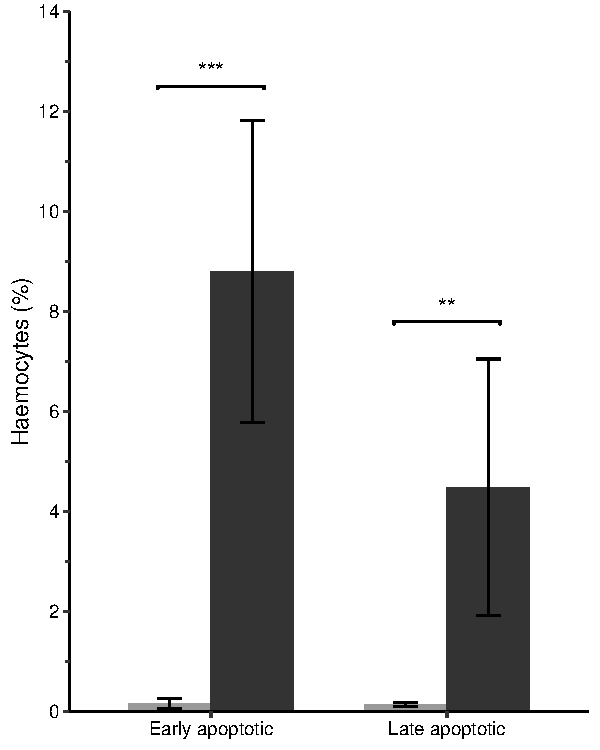
\includegraphics[width=0.5\textwidth]{figures/Method development/Apo15 pH.pdf}
    \caption{The mean percentage of early apoptotic (Apo15$^{+}$/ToPro3$^{-}$) and late apoptotic haemocytes (Apo15$^{+}$/ToPro3$^{+}$) after 15 minutes incubation in Anticoagulant Buffer (\, \protect\customgraybox, \ n=18) and non-adjusted Modified Alsever's Solution (\, \protect\darkgraybox, \ n=18). Error bars represent 95\% confidence intervals around group means. Asterisks *, **, *** denotes confidence level of one-tailed two sample t-test comparisons.}
    \label{fig:pH_Apo}
\end{figure}

Haemocytes that were incubated in the acidic MAS buffer showed a significant induction of apoptosis relative to samples kept in ACB. The mean percentage of early apoptotic haemocytes in naMAS were 53 times higher than in ACB (t(17) = 6.04, p<.001), while that of late apoptotic haemocytes were 31 times higher (t(17) = 3.57, p=.00117). The percentages of early and late apoptotic haemocytes in ACB were consistently low, with mean percentages of 0.165$\pm{0.2}$\% and 0.144$\pm{0.09}$\%, respectively.

\section{Development of a flow cytometric differential count}
This section presents the results of several experiments that were conducted in order to develop and validate a flow cytometric differential count of the cell types present in the haemolymph of \emph{M. edulis}. Section \ref{subsection:CytCar} presents a cytological characterization of the haemocytes according to i.a., cell size, granularity and staining affinities in accordance with the current scientific practice in invertebrate immunology. The flow cytometric characterization in section \ref{subsection:Results_FlowChar} presents the subpopulations of haemocytes that were separated according to FSC (relative size) and side scatter (internal complexity), and set these results in context of the cytologically defined cell types. The next section (\ref{subsection:evidence}) presents results from two experiments that were aimed to uncover the relationship between the cytologically defined cell types and the subpopulations discernible by light scatter measurements. Lastly, the gating strategy for the differential count is presented with proof of concept. The results are presented and discussed consecutively since each subsequent section builds on the preceding.

\subsection{Cytologic characterization of \emph{M. edulis} hemocyte subpopulations}
\label{subsection:Results_cytchar}
The hemolymph of \emph{Mytilus edulis} comprised a mixed population of cells differing in size, granularity, morphometrics and Wright's-Giemsa staining profiles. If the haemocytes were allowed to spread prior to fixation and staining, the diversity further expanded as cells took on a variety of shapes and/or developed cytoplasmic extensions. From these morphological criteria, a total of three distinct cell types could be identified by light microscopy.

Based on the basophilic or eosinophilic nature of their granules and other cytoplasmic contents, cytologic staining with 3 \% Wright's-Giemsa or the Hemacolor\textsuperscript{\textregistered} kit gave rise to two distinct staining profiles: basophilic and eosinophilic haemocytes. The cytoplasm of eosinophilic hemocytes (Figure \ref{fig:celltypes}, K-O) were densely packed with pink to dark purple granules of varying size and abundance. Hence, they are referred to as eosinophilic granulocytes herein. Their individual granules were usually not distinguishable in a non-spread state, but instead gave their cytoplasm an irregular pink color (Figure \ref{fig:celltypes}, K and O). These haemocytes had cell diameters in the range of 6-16 \micro m, with a mean of 9.06$\pm1.25$ \micro m. Two strikingly homogeneous features of this cell type was a small acentrically located nucleus, and a regular spherical outline in a non-spread state. With abundant pink cytoplasm making up the majority of the cells' surface area - even in the smallest specimens - the eosinophilic granulocytes could also be characterized by a low nuclear-cytoplasmic ratio (N:C ratio). If not fixed and stained before smearing - or within minutes of applying haemolymph to a glass slide - eosinophilic granulocytes were almost exclusively observed as spread cells. 

\begin{figure}[H]
    \centering
    \includegraphics[width=1.0\textwidth]{figures/Anatomy/cell types brightfield updated 2.pdf}
    \caption{100$\times$ brightfield micrographs of the three haemocyte types found in the haemolymph of \emph{Mytilus edulis}, fixed and stained on glass slides with the Hemacolor\textsuperscript{\textregistered} kit before the hemocytes had time to spread notably. \textbf{(A-E)} Blast-like hyaline basophils. \textbf{(F-J)} Basophilic granulocytes. \textbf{(K-O)} Eosinophilic granulocytes. Samples were withdrawn into \acrshort{mpss} (1:1), scale bars = 10 \micro m.}
    \label{fig:celltypes}
\end{figure}

Compared to the eosinophilic granulocytes, the basophilic hemocytes encompassed a more heterogeneous population. Common to all of them were a larger nucleus that occupied more of the cells' total surface area (higher N:C ratio). The shape of which varied from spherical to oval, or had a distinct bean-shaped or irregular outline. But judged from the morphological criteria of cell size, granularity and N:C ratio, there were essentially two distinct subpopulations of basophilic haemocytes: one population of small hyaline blast-like haemocytes (5.63 $\pm{0.72}$ \micro m) displaying only a marginal rim of dove blue cytoplasm and no apparent cytoplasmic granules (Figure \ref{fig:celltypes}, A-E), and one population of larger haemocytes (8.07 $\pm{1.25}$ \micro m), displaying abundant basophilic cytoplasm with varying degrees of cytoplasmic granulation and vacuolation (Figure \ref{fig:celltypes}, F-J). The basophillic granules appeared much smaller than those of the eosinophilic granulocytes, and were usually not very conspicuous unless haemocytes were subjected to osmotic swelling prior to fixation and staining. Under differential interference contrast (DIC) illumination however, their granules created highly irregular surface topographies in spread cells that could be observed without such treatment. On the basis of these morphological differences, the basophilic haemocytes were subdivided into blast-like haemocytes and basophilic granulocytes herein. 

\begin{figure}[H]
    \centering
    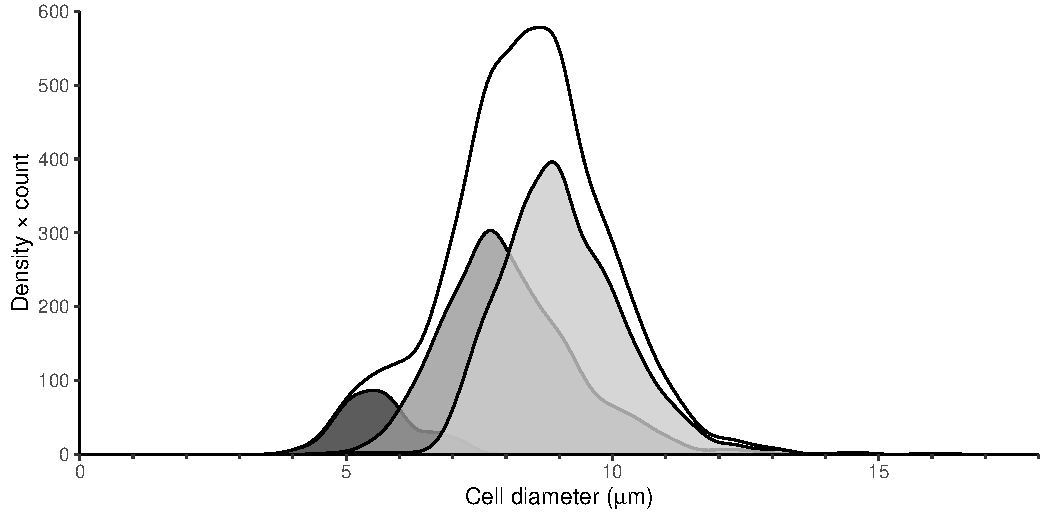
\includegraphics[width=1.0\textwidth]{figures/Anatomy/diameters scaled density plot.pdf}
    \caption{Size distribution of \protect\dimgraybox \ small blast-like basophils (n=154), \protect\lightgraybox \ basophilic granulocytes (n=821), \protect\lysegraabox \ eosinophilic granulocytes (n=1030) and \protect\whitebox \ the total haemocyte population of \emph{Mytilus edulis} (n=2005). The diameters of 100 formaldehyde-fixed haemocytes were measured in each of 20 individual mussels, and the density was scaled to the number of observations of each cell type.}
    \label{fig:Diameters}
\end{figure}

The size distributions of the three haemocyte types are shown as three kernel-smoothened density plots in Figure \ref{fig:Diameters}, together with that of the total haemocyte population. The densities have been scaled to the number of observations of each cell type, such that their relative proportions can be visualized. In the 20 adult mussels examined here, the small blast-like basophils were the least abundant cell type, making up 7.9 $\pm{5.6}$\% of the total haemocyte population. In 14 out of 20 mussels, the blast-like basophils were followed by the basophilic granulocytes, with a mean relative proportion of 40.7 $\pm{12.9}$\%. In spite of constituting similar proportions as the basophilic granulocytes in several mussels, the eosinophilic granulocytes were the most abundant cell type in the haemolymph of \emph{M. edulis}, constituting 51.5 $\pm{15.3}$\% of the total haemocyte population, on average. The relative proportions of basophilic and eosinophilic granulocytes did however vary to a large extent between individual mussels, as reflected by their standard deviations.

\subsection{Flow cytometric characterization of haemocyte subpopulations by light-scatter}
\label{subsection:Results_FlowChar}
A maximum of three distinct subpopulations could be separated according to Forwards scatter (FCS) vs. Side scatter (\acrshort{ssc}) in suspensions of living haemocytes. These comprised one subpopulation of events with low \acrshort{fsc}- and \acrshort{ssc}-values, one with high \acrshort{fsc}- and intermediate \acrshort{ssc}-values and one with high \acrshort{fsc} and \acrshort{ssc}. The aforementioned subpopulations correspond to clusters 1, 2 and 3 in Figure \ref{fig:fsc_vs_ssc}, where the haemocytes of three representative mussels have been displayed with \acrshort{ssc} on logarithmic and linear scales.

The adjunct histograms in Figure \ref{fig:fsc_vs_ssc}A and B clearly illustrates that the three clusters of events are separated according to log \acrshort{ssc}, while there is substantial overlap between cluster 2 and 3 with regard to \acrshort{fsc}. The latter feature was consistent across all mussels, while the degree of separation according to log \acrshort{ssc} was subject to individual variation. In this regard, the haemolymph sample presented in \ref{fig:fsc_vs_ssc}B represents a typical mussel, i.e., with cluster 2 and 3 incompletely separated according to log \acrshort{ssc}. The samples presented in \ref{fig:fsc_vs_ssc}A and C represents the extreme ends of this variation, with complete separation and complete overlap, respectively.

Since \acrshort{fsc} and \acrshort{ssc} can be interpreted as relative measures of cell size and internal complexity, these results suggests that the haemolymph of \emph{M. edulis} are comprised of three cell types that are distinguishable according to size and internal complexity. The events populating cluster 1 exhibited low \acrshort{fsc}- and \acrshort{ssc}-values relative to cluster 2 and 3, indicating that it is populated by haemocytes that are both smaller and less complex than the rest of the haemocytes. If \acrshort{ssc} is interpreted more specifically in terms of haemocyte characteristics, the events populating cluster 2 and 3 most likely correspond to large semi-granular haemocytes and large granulocytes, respectively.

\begin{figure}[ht!]
    \centering
    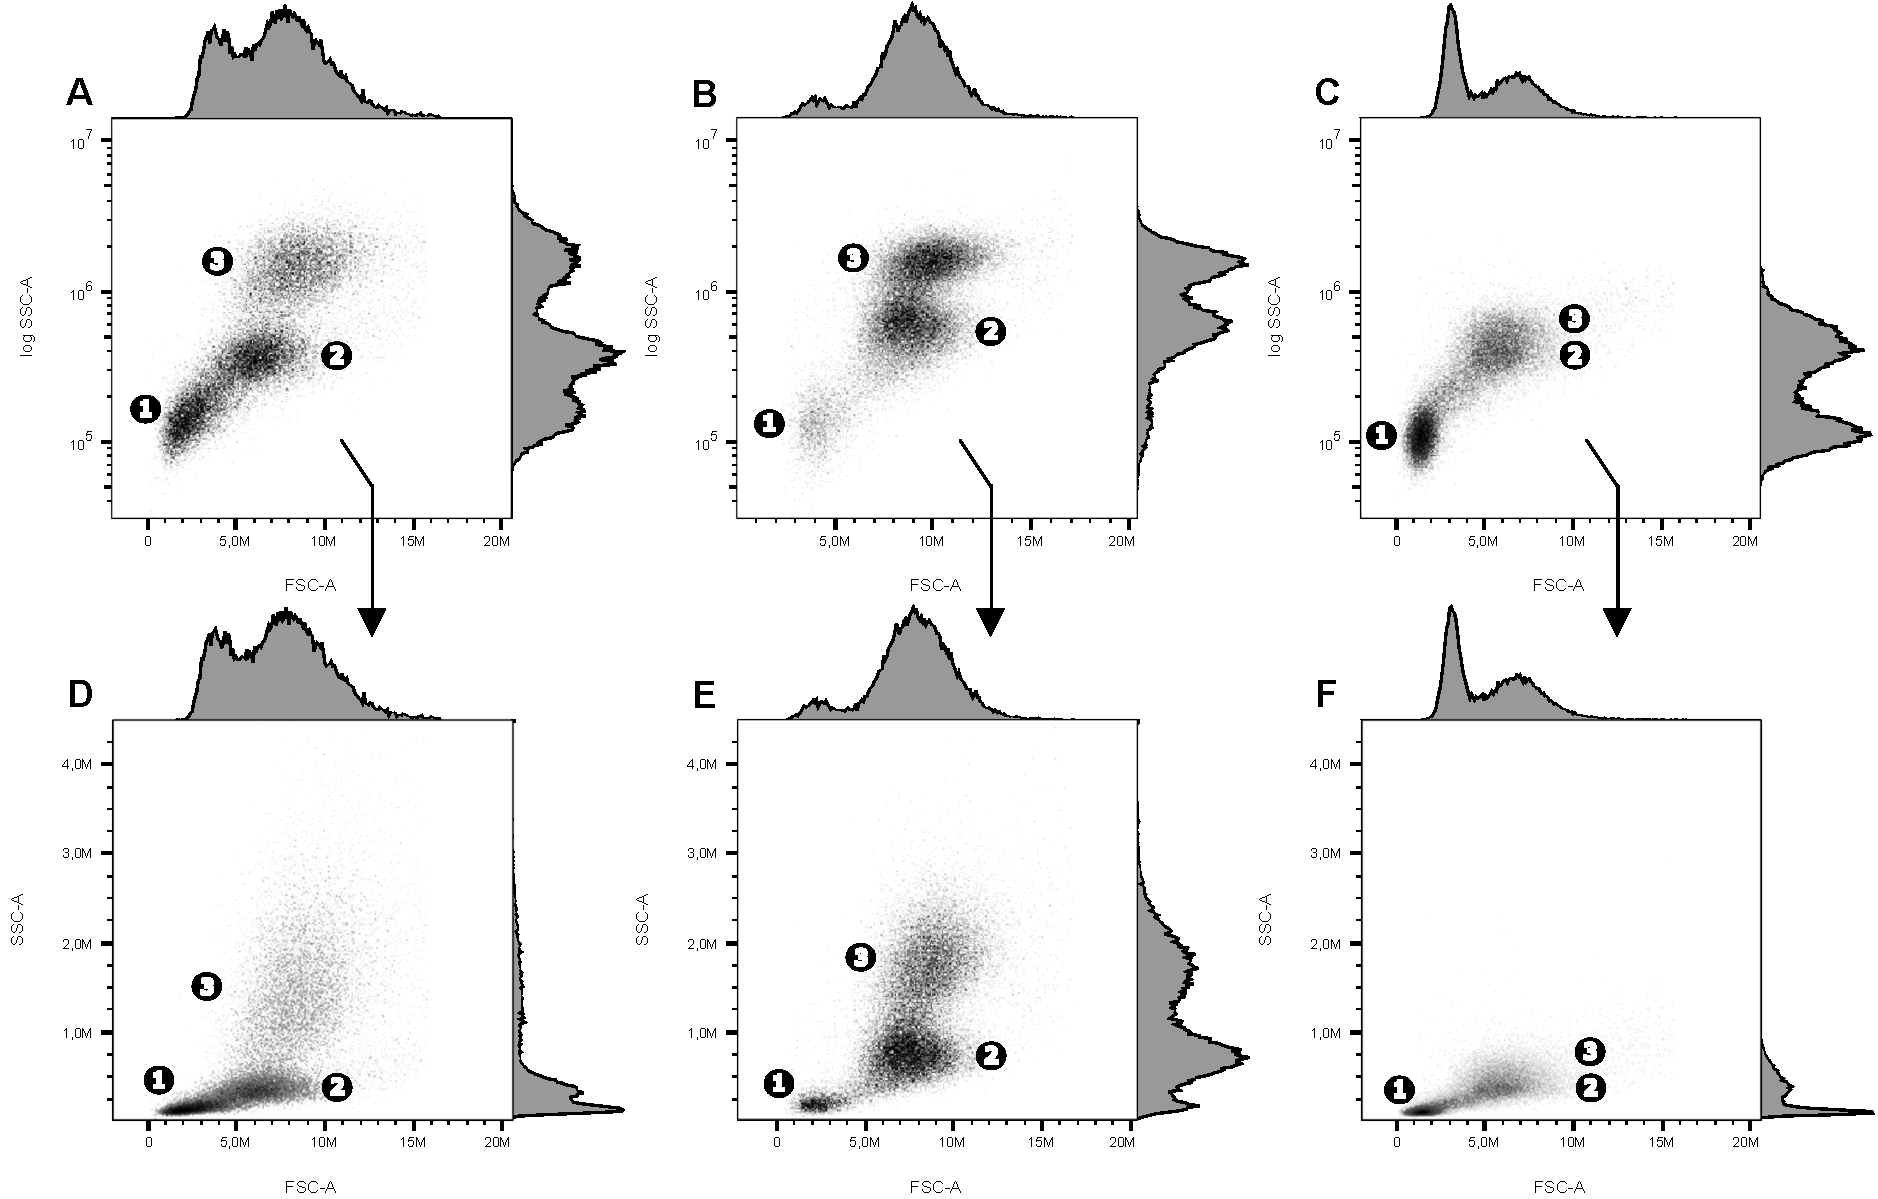
\includegraphics[width=1.0\textwidth]{figures/Gating strategy/30k scatter profiles musc.pdf}
    \caption{\textbf{Haemocyte subpopulations distinguishable according to \acrshort{fsc} and \acrshort{ssc} measurements with the BD Accuri C6 Plus Benchtop Flow Cytometer.} The light-scatter profiles of three representative adult mussels are displayed with \acrshort{ssc} on logarithmic \textbf{(A-C)} and linear \textbf{(D-F)} scales to illustrate the observed variation in the degree of separation between cluster 2 and 3. Adjunct histograms were included to underline the degree of separation from the individual parameters.}
    \label{fig:fsc_vs_ssc}
\end{figure}

\subsection{Relating cytologically defined cell types to light-scatter profiles}
\label{subsection:evidence}
\subsubsection{Flow cytometric characterization of haemocytes pre-separated by isopycnic centrifugation }
Formaldehyde-fixed haemocytes separated into three distinct cell-bands on the 15/33\%, 38/43\% and 43/90\% gradient interfaces of the discontinuous Percoll gradients. As shown in Figure \ref{fig:Percoll-tubes}, the two upmost bands exhibited a similar blue coloration, while the band located on the 43/90\% interface had a darker purple color. The latter consisted of 96.9$\pm{0.9}$\% eosinophilic granulocytes, with a few basophillic granulocytes scattered among them. From the cell bands located at the 15/33\% interface, a populations of 96.3$\pm{0.2}$\% basophillic haemocytes were isolated. The majority of these cells were basophilic granulocytes (87.5$\pm{1.2}$\%), with a smaller fraction of blast-like basophils (8.8$\pm{1.5}$\%). The middle bands did not yield any of the cell types in high purity, but were predominantly populated by basophilic granulocytes (72.7$\pm{1.5}$\%) with numerous small dark granules.

\begin{figure}[H]
    \centering
    \includegraphics[width=.75\textwidth]{figures/Method development/Percoll tubes.pdf}
    \caption{\textbf{Formaldehyde-fixed haemocytes pre-stained with Giemsa were separated by isopycnic centrifugation on discontinuous Percoll gradients.} Haemocytes settled into three distinct cell bands on the 15/33\%, 38/43\% and 43/90\% gradient interfaces.}
    \label{fig:Percoll-tubes}
\end{figure}

The light scatter profiles of the three isolated cell fractions are depicted in Figure \ref{fig:Percoll-dotplots}, together with that of the unseparated haemocytes. As shown in Figure \ref{fig:Percoll-dotplots}A, the pooled haemocyte were not readily distinguishable as three separate subpopulations prior to centrifugation. Since the relative size and complexity of the three cell types vary slightly between individual mussel, this is a common phenomenon when haemolymph from two or more mussels are pooled together. A more distinct clustering was however seen among haemocytes isolated from the middle cell-band (\ref{fig:Percoll-dotplots}C), where the relative proportions of eosinophilic granulocytes (18.4\%) and blast-like basophils (7.8\%) were lower.

\begin{figure}[H]
    \centering
    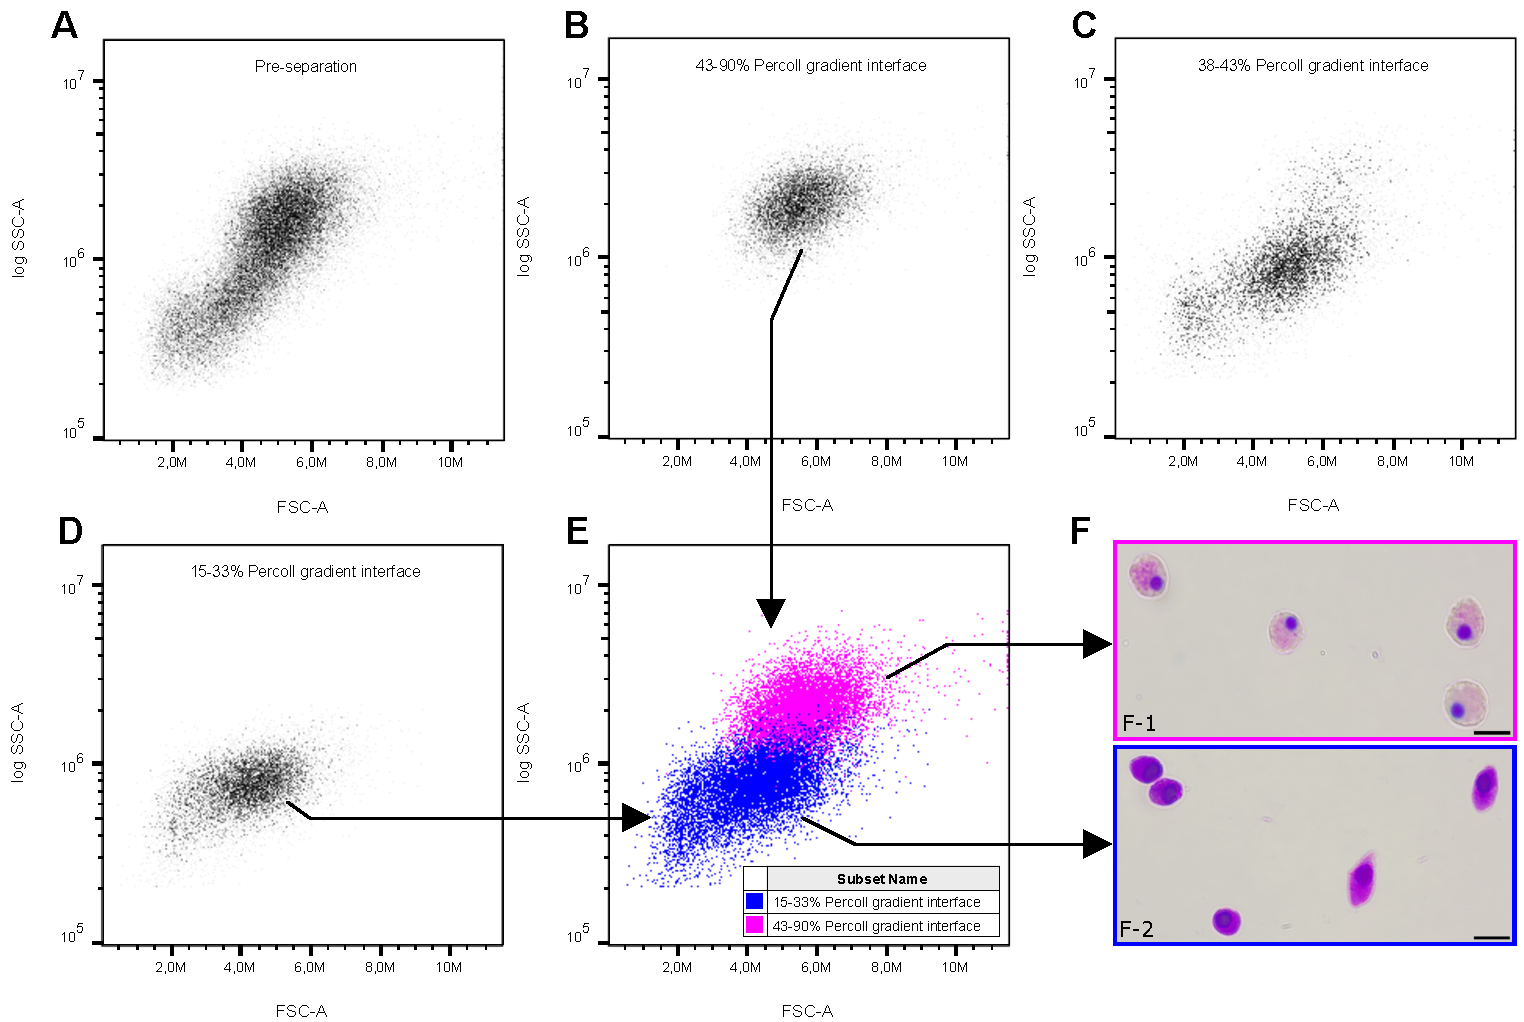
\includegraphics[width=1.0\textwidth]{figures/Method development/PERCOLL SEP II.pdf}
    \caption{\textbf{Flow cytometric analysis of the isolated cells types of \emph{M. edulis} haemolymph after separation by isopycnic centrifugation.} Two pools of formaldehyde-fixed haemocytes were separated by density-dependent centrifugation after the method of Friebel and Renwrantz (1994), and the isolated fractions were analyzed by flow cytometry and light microscopy. FSC vs. log SSC density plots depicts one of the pools prior to centrifugation \textbf{(A)} and after separating into three distinct cell-bands on the gradient interfaces \textbf{(B-D)}. The enriched fractions (> 96\%) of eosinophilic granulocytes \textbf{(B)} and basophilic haemocytes \textbf{(D)} are overlayed in \textbf{(E)}, with micrographs of the respective layers presented in \textbf{(F)}. F-1: eosinophilic granulocytes; F-2: basophilic granulocytes; scale bars = 10 \micro m. }
    \label{fig:Percoll-dotplots}
\end{figure}

The eosinophilic granulocytes formed a dense cluster of events exhibiting high FSC- and SSC-values (Figure \ref{fig:Percoll-dotplots}B). This is consistent with the expected light scatter profile of this cell type, since they represent highly granulated cells with large cell diameters. The two basophilic cell types from the upper cell band were unambiguously separated from the eosinophilic granulocytes according to SSC, where only a small number of cells exceeded values > 1$\times 10^{6}$ (Figure \ref{fig:Percoll-dotplots}D). This relationship is clearly demonstrated by the overlayed dotplot in Figure \ref{fig:Percoll-dotplots}E, where the eosinophilic granulocytes are shown in pink.

\subsubsection{Identification of eosinophilic granulocytes by eosin fluorescence}
Formaldehyde-fixed haemocytes stained with 0.5\% eosin were separated into distinct eosin$^{bright}$ and eosin$^{dim}$ populations by flow cytometric measurements of eosin fluorescence (Figure \ref{fig:eosin_exp2}B and C). The degree of separation varied to a large extent between individual mussels, but the \acrshort{mfi} of eosin$^{bright}$ events were 11$\pm{9}$ times higher than that of eosin$^{dim}$ events on average. The difference in fluorescent intensity between eosinophilic and basophilic granulocytes is illustrated in Figure \ref{fig:Eosin_fluorescence_B2A}, where Giemsa-stained haemocytes have been imaged by epifluorescence microscopy with a B-2A filtercube (Em: $\geq$ 515 nm; exposure: 250 msec; gain: 3.4).

\begin{figure}[H]
    \centering
    \begin{subfigure}[b]{.45\textwidth}
        \centering
        \includegraphics[width=\textwidth]{figures/Method development/B2A eosin fluorescence/Epi eosin fluorescence.pdf}
        \caption{Hemocytes imaged under brightfield illumination.}
        \label{ffig:a}
    \end{subfigure}
    \hfill
    \begin{subfigure}[b]{.45\textwidth}
        \centering
        \includegraphics[width=\textwidth]{figures/Method development/B2A eosin fluorescence/Brightfield eosin fluorescence.pdf}
        \caption{Haemocytes imaged by epifluorescence microscopy with a B-2A filtercube.}
        \label{ffig:b}
    \end{subfigure}
    \caption{\textbf{Eosinophilic granulocytes are distinguished from the two basophilic cell types according to eosin fluorescence ($\geq$ 515 nm).} Formaldehyde-fixed haemocytes stained in 0.5\% eosin and 3\% Giemsa were imaged at $\times$60 magnification under \textbf{a)} brightfield illumination and \textbf{b)} by epifluorescence microscopy with a B-2A filter cube. The slide was mounted with Eukitt\textsuperscript{\textregistered} and coverslipped prior to microscopy. Eo: eosinophilic granulocyte; B: basophilic haemocyte; scale bars = 10 \micro m. }
    \label{fig:Eosin_fluorescence_B2A}
\end{figure}

The pooled sample depicted in Figure \ref{fig:eosin_exp2}A were unambiguously separated into three distinct haemocyte subpopulations according to FSC and SSC. These subpopulations are equivalent to cluster 1-3 in samples of living haemocytes (see Figure \ref{fig:fsc_vs_ssc}). When the eosin$^{bright}$ events were back-gated to bivariate plots of FSC vs. SSC, they invariably corresponded to the subpopulation with high FSC- and SSC-values, i.e., cluster 3. (see Figure \ref{fig:eosin_exp2}D). This is clearly demonstrated by comparing Figure \ref{fig:eosin_exp2}A and D, where the eosin$^{bright}$ events are shown in pink.

The correlation between eosin$^{bright}$ events (\%) and the percentage of eosinophilic granulocytes were analyzed by simple linear regression on order to verify the linearity of response. The analysis showed that eosin$^{bright}$ events (\%) recorded by flow cytometry significantly predicted the percentage of eosinophilic granulocytes($\beta$ = 1.06656, 95\% CI [0.96, 1.17], t(8) = 23.3, p<.001), with a mean absolute error of 1.71$\pm{1.6}$\%. The data is presented in Figure \ref{fig:eosin_exp2}E, together with the fitted linear regression model (R$^{2}$ = 0.99, F(1, 8) = 541, p<.001).

\begin{figure}[H]
    \centering
    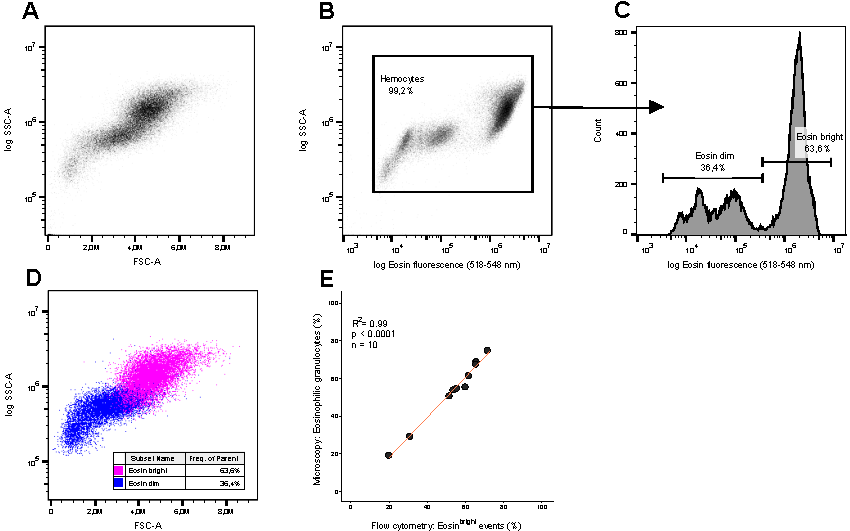
\includegraphics[width=1.0\textwidth]{figures/Method development/Eosin with method validation.pdf}
    \caption{\textbf{Identification eosinophilic granulocytes on FSC vs. SSC dotplots according to log eosin fluorescence (518-548 nm).} Ten formaldehyde-fixed haemolymph samples were stained with 0.5\% eosin and recorded on the flow cytometer right thereafter \textbf{(A)}. Haemocyte events were gated according to log eosin fluorescence vs. SSC-A \textbf{(B)} and the eosin$^{bright}$ events were gated univariately \textbf{(C)}. The eosin$^{bright}$ events were back-gated to show their light scatter profile relative to eosin$^{dim}$ events \textbf{(D)}. The simple regression of eosin$^{bright}$ events (\%) vs. eosinophilic granulocytes (\%) determined from 1000-cell differential counts are shown in \textbf{(E)}, regression line: y$_{i}$ = -3.20042 + 1.06656x$_{i}$.}
    \label{fig:eosin_exp2}
\end{figure}

\subsection{Flow cytometric differential haemocyte count}


\begin{figure}[H]
    \centering
    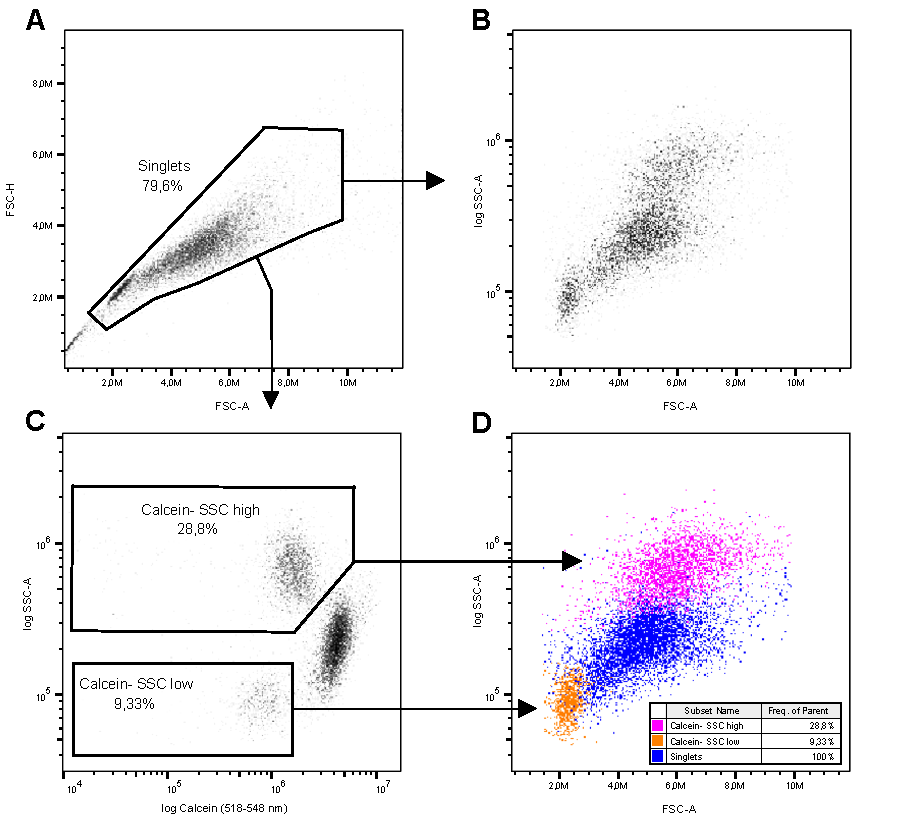
\includegraphics[width=1.0\textwidth]{figures/Gating strategy/GatestratGY SSC Calcein PNG.pdf}
    \caption{ \textbf{Differential haemocyte count gating strategy}.}
    \label{fig:DHC_gatestrat}
\end{figure}





\begin{figure}[H]
    \centering
    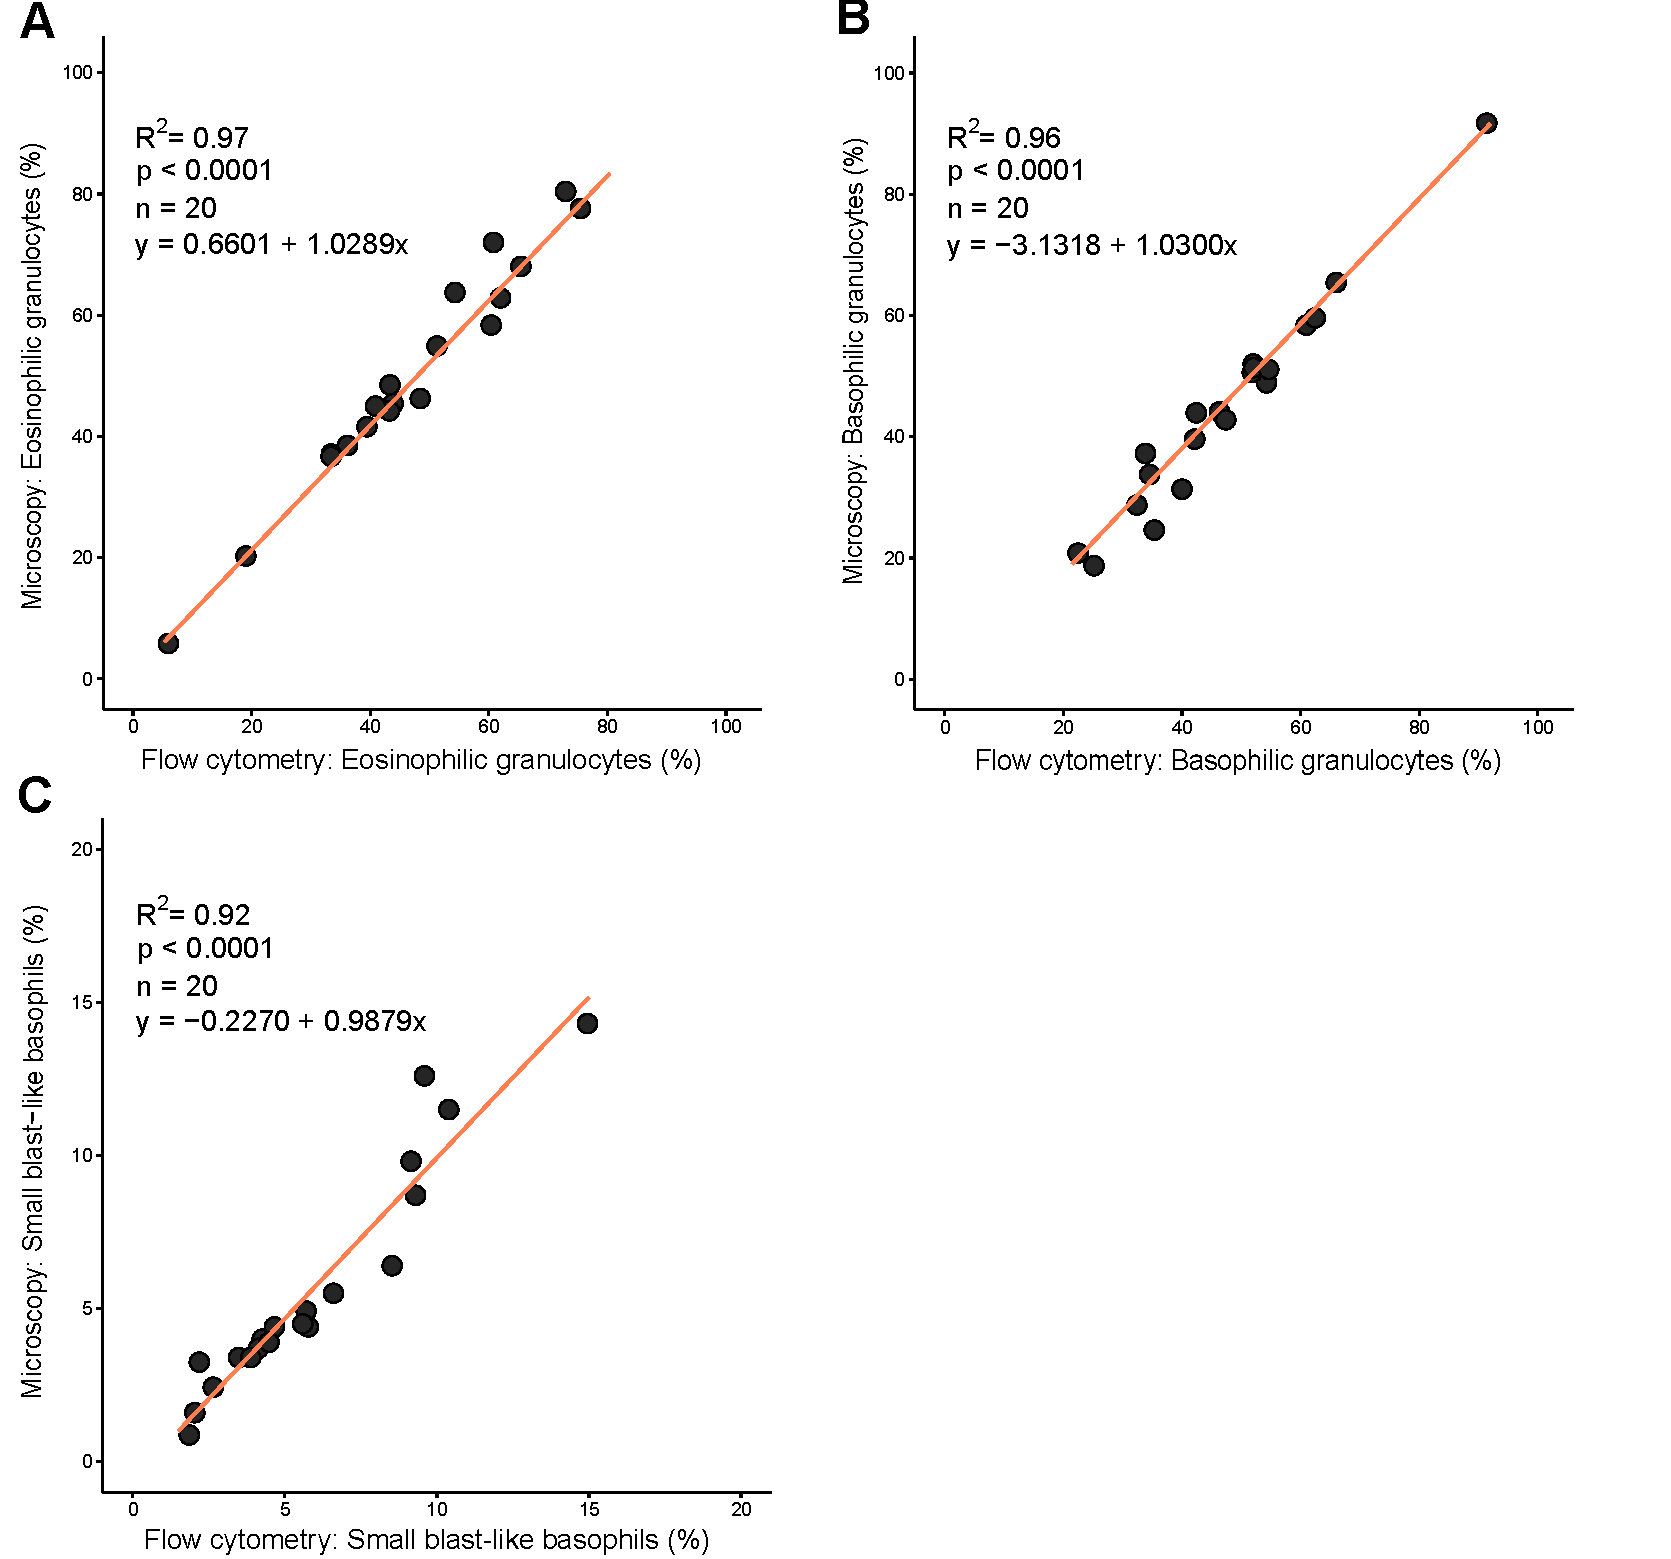
\includegraphics[width=1.0\textwidth]{figures/Gating strategy/SSC Calcein validation.pdf}
    \caption{Correlation between the percentages of eosinophilic granulocytes \textbf{(A)}, basophilic granulocytes \textbf{(B)} and small blast-like basophils \textbf{(C)} from differential haemocyte counts performed by microscopy and flow cytometry (n=20). The three cell types were were differentiated according log SSC-A vs. log Calcein fluorescence (518-538 nm), as shown in the gating strategy in Figure 3.12. }
    \label{fig:DHC_lin}
\end{figure}

%  A: f(x) = -0.22708 + 0.98789x, 95\% CI [0.89148, 1.0842], MAE = 0.5755
% BG: f(x) = -3.13182 + 1.03003x, 95\% CI [0.96733, 1.0927], MEA = 2.263
% Eo: f(x) =  0.66011 + 1.02894x, 95\% CI [0.97425, 1.0836], MEA = 2.457


\newpage




\section{Scoring of necrotic haemocytes by flow cytometry}
\subsection{Determination of optimal TO-PRO-3 Iodide staining concentration}
Viable and \ce{MeOH}-killed haemocytes could be separated according to TO-PRO-3 Iodide fluorescence in the whole range of tested concentrations (30 nM - 8 \micro M). As shown in Figure \ref{fig:ToPro3_stain_opt}B, the resolution between ToPro3$^{-}$ and ToPro3$^{+}$ events increased with the TO-PRO$^{TM}$-3 Iodide concentration according to the log-logistic function shown in (\ref{eq:fitted.LL4}), with a marked stagnation > 1.2 \micro M. The model explained almost all the variation in the dataset (Pseudo-R$^{2}$ = 0.99, see table \ref{tb:loglogistic_ToPro3}), and should therefore be a good predictor of the expected resolution between necrotic and viable haemocytes in the tested range of TO-PRO$^{TM}$-3 Iodide.

\begin{equation}
\label{eq:fitted.LL4}
y_{i} = \dfrac{9890700}{1 + (x_i / 0.41655)^{-0.94088}} + \epsilon_i
\end{equation}

\begin{figure}[h]
    \centering
    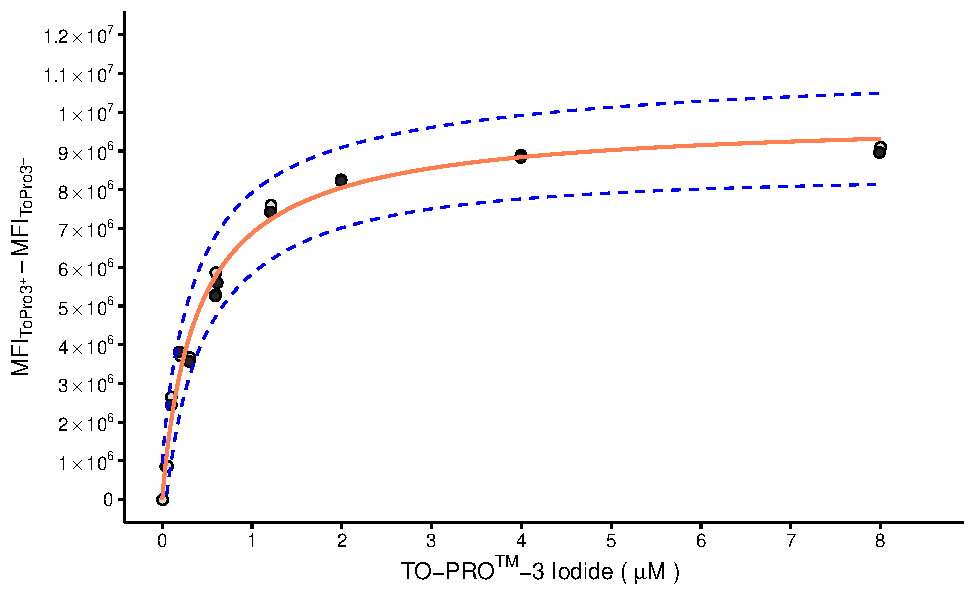
\includegraphics[width=1.0\textwidth]{figures/Method development/ToPro3 LL4.pdf}
    \caption{\textbf{Experimental determination of the optimal TO-PRO$^{TM}$-3 Iodide concentration for a dye exclusion test of membrane integrity}. 10 aliquots of pooled methanol-killed (70\% \ce{MeOH}, 30 min) and viable haemocytes (1:1) were stained with different concentrations of TO-PRO$^{TM}$-3 Iodide (30 nM - 8 \micro M). 640 nm-exited fluorescence from \acrshort{dsdna}-bound TO-PRO$^{TM}$-3 Iodide were collected on the FL4 detector (675/25 nm) of the BD Accuri C6 Plus flow cytometer, recording 10.000 events from each sample after 15 and 30 minute incubation. \textbf{A)} ToPro3$^{-}$ and ToPro3$^{+}$ events were gated on log scale for each sample, \textbf{B)} and their difference in mean fluorescent intensity (MFI) after 15 (\protect\lysegraacircle) and 30 minutes (\protect\darkgraycircle) of incubation were plotted against the concentration of TO-PRO$^{TM}$-3 Iodide. Red line: fitted log-logistic regression model; blue dashed lines: prediction intervals.}
    \label{fig:ToPro3_stain_opt}
\end{figure}

The predicted difference in \acrshort{mfi} at 1.2 \micro M was 7.220.000 (arbitrary units), 95\% PI[6.170.000, 8.260.000]. Since the slope of function \ref{eq:fitted.LL4} decreased rapidly for x > 0.6, the predicted difference in MFI at x = 1.2 \micro M was contained within the prediction intervals for the rest of the function's range. Furthermore, the MFI of the ToPro3$^{-}$ populations increased abruptly at concentrations $\geq$ 2 \micro M (see Table \ref{tb:ToPro3_stainopt}), indicating a potential cytotoxic effect of either TO-PRO$^{TM}$-3 Iodide or the \acrshort{dmso} solvent at high concentrations.

Taken together, these results suggested that the potential gain from increasing the staining concentration above 1.2 \micro M was limited, and not completely free of risk. The resolution between viable and necrotic haemocytes was for all practical purposes sufficient in the range of 300 nm - 1.2 \micro M, but the resolution at 1.2 \micro M would simplify gating on a logarithmic scale. 1.2 \micro M TO-PRO$^{TM}$-3 Iodide was therefore preferred for scoring necrotic haemocytes by flow cytometry, together with 50 nM Calcein AM.

The results were also unambiguous regarding the incubation period. According to Figure \ref{fig:ToPro3_stain_opt}B, the resolution between viable and necrotic cells did not increase after the initial 15 minute incubation period. The MFI of necrotic haemocytes did increase somewhat in the extended incubation period, but the resolution remained unchanged due to a concurrent proportional increase among the viable haemocytes (see table \ref{tb:ToPro3_stainopt}, Appendix B). Extending the incubation period beyond 15 minutes would therefore be of little use.

\subsection{Gating strategy}
The finalized quadrant gating strategy for the Calcein AM/TO-PRO$^{TM}$-3 Iodide membrane integrity assay is presented in Figure \ref{fig:TP3_Calcein_gating_strat}. The four plots (A-D) represent samples of viable and methanol-killed haemocytes in equal proportions (A, unstained control; B, Calcein FMO; C, TO-PRO$^{TM}$-3 Iodide FMO; D, Calcein/TO-PRO$^{TM}$-3 Iodide). Unstained controls were used to establish a tentative lower left quadrant gate (Calcein$^{-}$ ToPro3$^{-}$) for non-cellular events. This quadrant was expanded in both directions to include all Calcein$^{-}$ events of the Calcein FMOs and all the ToPro3$^{-}$ events of the TO-PRO$^{TM}$-3 Iodide FMOs (see Figure \ref{fig:TP3_Calcein_gating_strat}B and C). When the double stained samples were run, the viable and methanol-killed haemocytes populated the upper left and lower right quadrants, exclusively (see Figure \ref{fig:TP3_Calcein_gating_strat}D).

\begin{figure}[h]
    \centering
    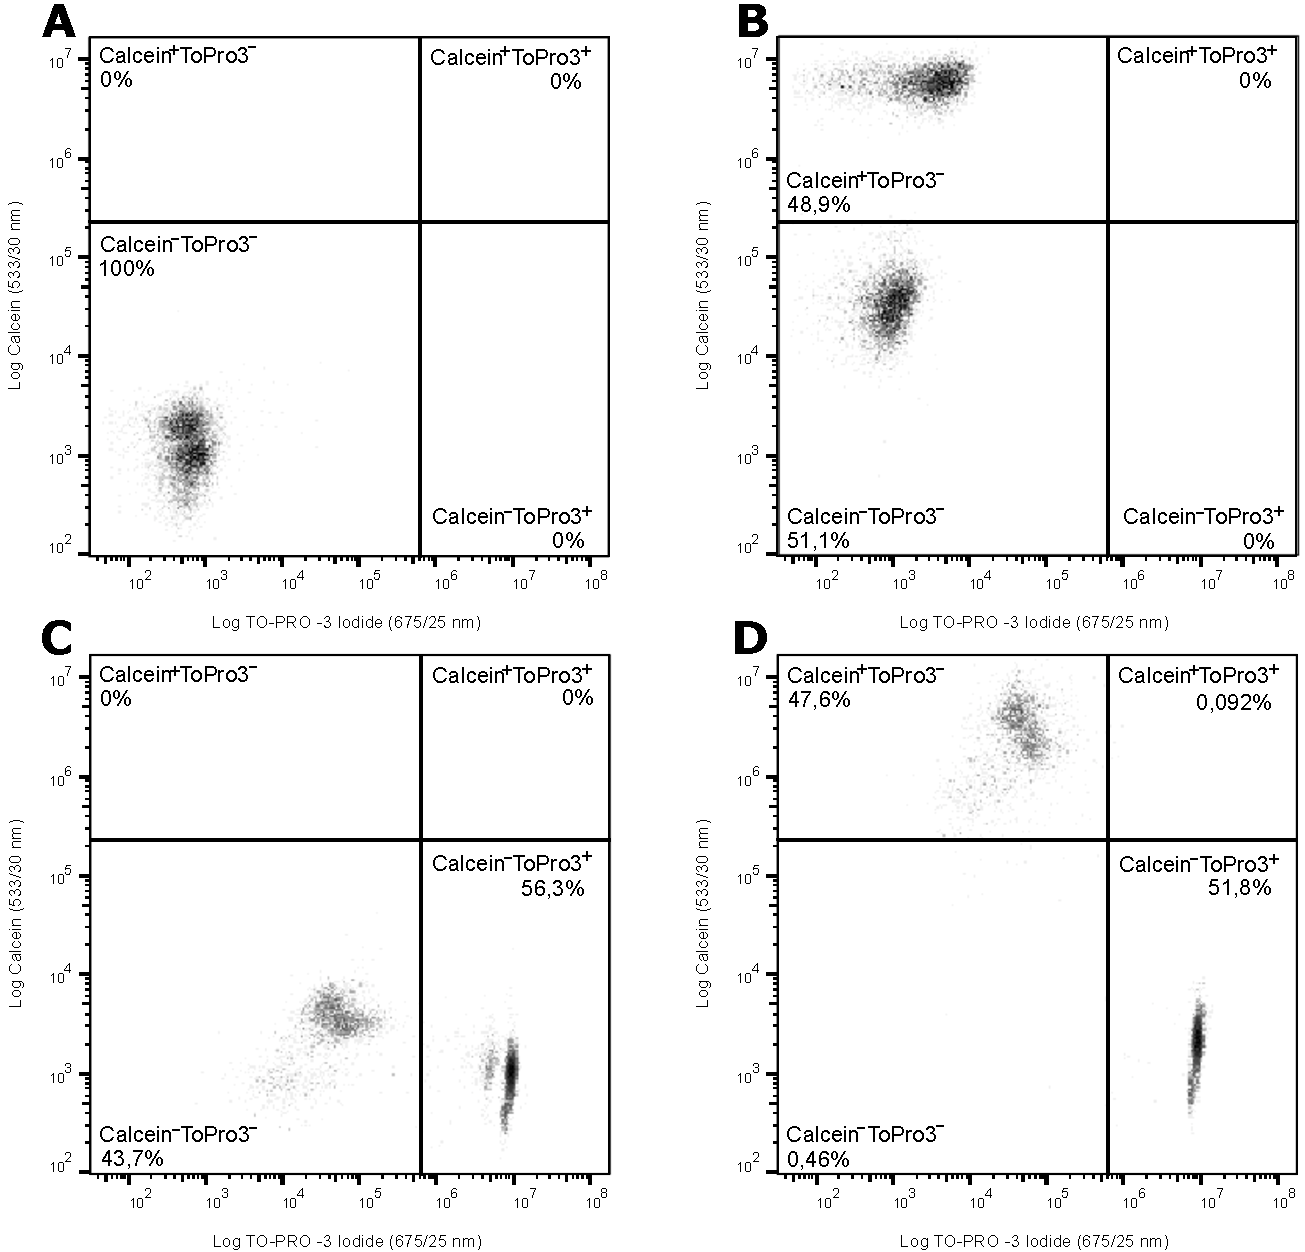
\includegraphics[width=.7\textwidth]{figures/Gating strategy/ToPro3 CAM gating strategy.pdf}
    \caption{\textbf{FL1 (533/30 nm) vs. FL4 (675/25 nm) quadrant gating for flow cytometric scoring of necrotic (Calcein$^{-}$ ToPro3$^{+}$) an viable (Calcein$^{+}$ ToPro3$^{-}$) haemocytes.} By preparing a pool of \ce{MeOH}-killed and newly withdrawn haemocytes in antiaggregative buffer (\acrshort{acb}), gates were drawn according to the florescent profiles of \textbf{A)} Unstained controls, \textbf{B)} Calcein \acrshort{fmo}s, \textbf{C)} TO-PRO$^{TM}$-3 Iodide FMOs and \textbf{D)} aliquotes stained with both probes.}
    \label{fig:TP3_Calcein_gating_strat}
\end{figure}


\subsection{Method validation}
Simple linear regression was used to examine the correlation between results obtained by epifluorescent microscopy and the flow cytometric gating strategy presented in Figure \ref{fig:TP3_Calcein_gating_strat}. It was found that the established quadrant gating strategy significantly predicted the the percentage of ToPro3$^{+}$ haemocytes in samples scored by epifluorescent microscopy ($\beta$ = 0.98818, t(8) = 32.8, p<.001). The data is presented in Figure \ref{fig:method_val_1}, together with the fitted linear regression model (R$^{2}$ = 0.99, F(1, 8) = 1059, p<.001).

\begin{figure}[b]
    \centering
    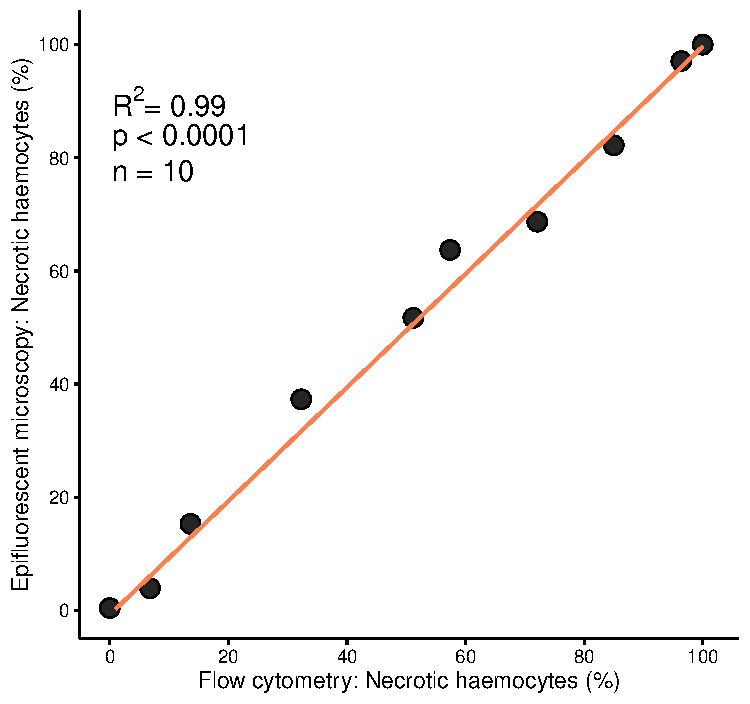
\includegraphics[width=.5\textwidth]{figures/Method development/FCM FM lin reg.pdf}
    \caption{\textbf{Correlation between necrotic haemocyte percentages scored by flow cytometry and epifluorescent microscopy.} 10 samples of freshly withdrawn haemocytes (\acrshort{acb}, 1:1) were mixed with methanol-killed haemocytes in semi-random proportions (0-100\%), stained with Calcein AM (50 nM) and TO-PRO$^{TM}$-3 Iodide (1.2 \micro M) and the percentage of necrotic haemocytes (\%) were scored by both flow cytometry and epifluorescent microscopy. Each datapoint represents one scored sample. Red line: fitted linear regression model.}
    \label{fig:method_val_1}
\end{figure}